\chapter{Model danych}
\label{chap5}
%Umiścić na diagramach rekacje identyfikujące dla encji typ_zadania, adres_pracownika, składka pracownika, rachunek

%TODO usunac kropke nad z w budzet
%TODO ubezpieczenia dobrowolne w encji UMOWA
%TODO typ zadania nie nullowany w zadaniu
%wynagrodzenie obowiazkowe w umowie
\section[Model logiczny][Model logiczny]{Model logiczny}
Jednym z pierwszych etapów projektowania bazy danych jest stworzenie modelu logicznego. Prezentuje on ogólną koncepcję bazy, niezwiązaną z żadnym konkretnym systemem zarządzania bazą danych. Najpopularniejszym przykładem modelu logicznego jest model związków encji. Polega on na przedstawieniu zagadnienia za pomocą encji, ich atrybutów oraz związków pomiędzy nimi. Na rysunkach \ref{logiczny1}, \ref{logiczny2}, \ref{logiczny3} przedstawiono diagramy związków encji dla projektowanego systemu.

\begin{figure}[tdh]
    \begin{center}
	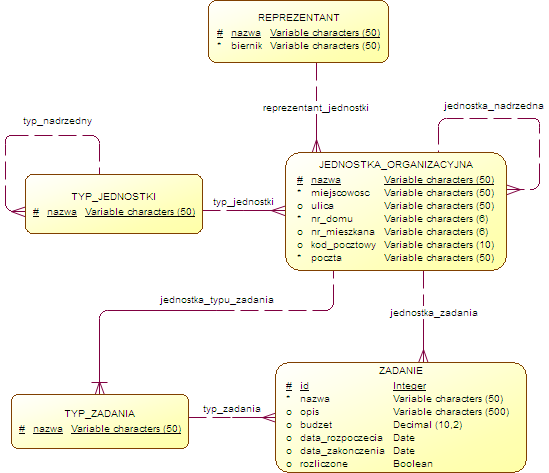
\includegraphics[scale=.8]{img/logiczny1.png}
	\caption{Model związków encji opisujący strukturę organizacyjną instytucji}
	\label{logiczny1}
    \end{center}
\end{figure}
\begin{figure}[tdh]
    \begin{center}
	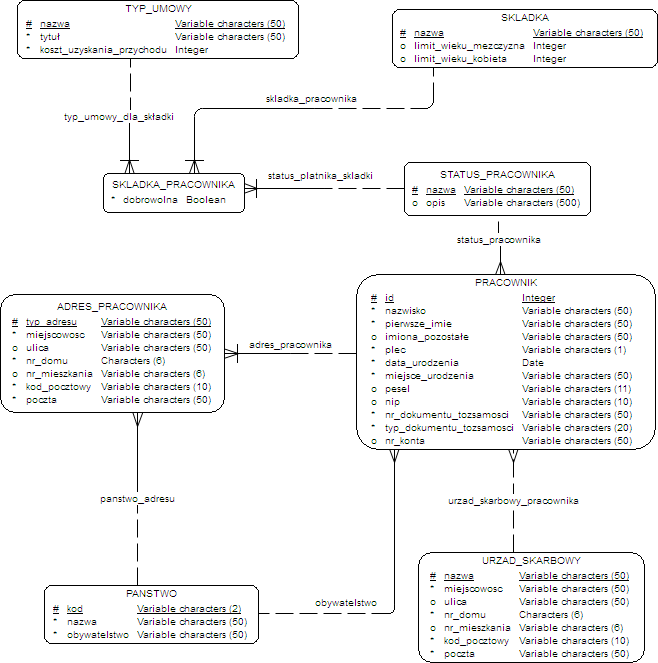
\includegraphics[scale=.8]{img/logiczny2.png}
	\caption{Model związków encji opisujący pracownika}
	\label{logiczny2}
    \end{center}
\end{figure}
\begin{figure}[]
    \begin{center}
	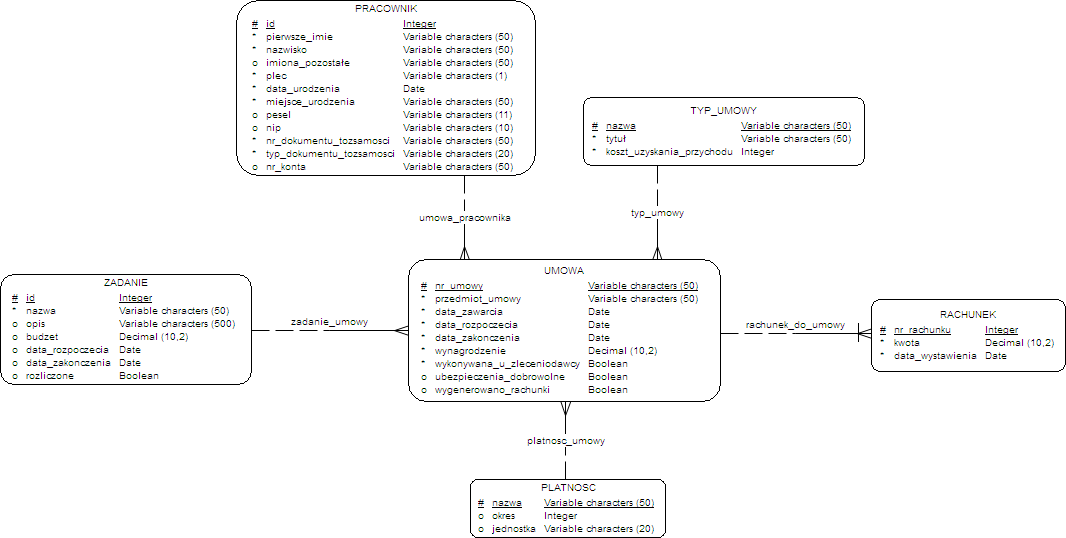
\includegraphics[scale=.8,angle=-90]{img/logiczny3.png}
	\caption{Model związków encji opisujący umowę}
	\label{logiczny3}
    \end{center}
\end{figure}

\subsubsection{Pracownik}
Encja ta zawiera informacje dotyczące pracownika, który może być zatrudniany na umowy-cywilno prawne. Powstała na podstawie wymagań opisanych w rozdziale \ref{pracownicy}. Podstawowymi atrybutami tej encji są nazwisko i imiona pracownika. Z racji, że w zależności od sytuacji raz posługujemy się jedynie pierwszym imieniem, innym zaś razem zachodzi potrzeba wymienienia wszystkich imion, encja ta posiada dwa atrybuty: pierwsze imię oraz imiona pozostałe. Kolejnymi atrybutami pracownika są płeć, data urodzenia, miejsce urodzenia, numery PESEL oraz NIP, numer konta oraz numer dokumentu tożsamości. Dokumentem takim może dowód osobisty lub paszport  (w przypadku obcokrajowców). Powstała więc konieczność wprowadzenia kolejnego atrybutu jakim jest typ dokumentu tożsamości.

W przypadku tej encji nie udało się znaleźć naturalnego identyfikatora. Nie może nim być zbiór atrybutów: nazwisko, pierwsze imię oraz imiona, gdyż niewykluczona jest sytuacja, że w systemie znajdzie się dwóch pracowników nazywających się tak samo. Funkcji takiej nie mogą także pełnić numery PESEL oraz NIP. Nie ma przecież gwarancji na ich unikalność. Wprowadzono więc sztuczny identyfikator w postaci atrybutu id.

\subsubsection{Adres Pracownika}
Encja ta powstała z konieczności umożliwienia posiadania przez pracownika dwóch adresów: wykorzystywanego w celach podatkowych oraz korespondencyjnego, w przypadku gdy ten drugi różniłby się od pierwszego. Stąd też podstawowym atrybutem tej encji jest typ adresu (w celach podatkowych lub korespondencyjny). Oprócz tego posiada takie atrybuty jak miejscowość, ulica, numer domu, numer mieszkania, kod pocztowy i poczta. Na uwagę zasługują takie atrybuty jak ulica i numer mieszkania. Nie są one obowiązkowymi elementami adresu, gdyż ulice nie występują w każdej miejscowości (szczególnie na wsiach, ze względu małą liczbę mieszkańców, nie ma potrzeby ich wprowadzania), a numerów mieszkania nie posiadają m. in. domy jednorodzinne. Kolejną istotną kwestią jest rozdzielenie atrybutów miejscowość i poczta. Wiele modeli niesłusznie zakłada, że atrybuty te są tożsame. Niestety, nie jest to regułą - nie każda miejscowość jest siedzibą poczty.
W przypadku tak skonstruowanej encji udało się znaleźć naturalny identyfikator. Jest to para: relacja z encją pracownik oraz atrybut typ adresu.

\subsubsection{Państwo}
Jest to encja słownikowa. Pojawiła się w systemie z dwóch powodów. Pierwszym z nich jest konieczność przechowywania informacji o obywatelstwie pracownika  (stąd relacja ,,obywatelstwo''). Drugim powodem jest obecność państwa w adresie. Atrybutami państwa są jego nazwa (np. Polska) oraz nazwa obywatelstwa (np. polskie). Jako unikalny identyfikator państwa wybrano dwuliterowy kod ISO-3166-1\cite{panstwa} (np. PL).

\subsubsection{Urząd Skarbowy}
Encja ta opisuje urząd skarbowy właściwy dla pracownika. Podstawowym jej atrybutem jest nazwa. Pełni ona funkcję unikalnego identyfikatora tej encji. Zawiera ona zazwyczaj informacje o miejscowości oraz numerze urzędu skarbowego (np. Pierwszy urząd skarbowy w Lublinie). Nie jest to jednak regułą. Zdarza się, że zamiast numeru występuje nazwa dzielnicy czy nazwa własna urzędu skarbowego. Nie udało się więc rozbicie tego atrybutu na mniejsze części (w szczególności wyodrębnienie atrybutu numer urzędu skarbowego). Pozostałymi atrybutami urzędu skarbowego są dane adresowe, czyli miejscowość, ulica, numer domu, numer mieszkania, kod pocztowy i poczta.

\subsubsection{Status pracownika}
Encja ta opisuje status pracownika w świetle obowiązków odprowadzania składek na różnego rodzaju ubezpieczenia i fundusze. Przykłady takich statusów zostały opisane w sekcji \ref{przykladyOsob}. Atrybutami tej encji są nazwa oraz opis. Nazwa jest ponadto jej unikalnym identyfikatorem.

\subsubsection{Jednostka organizacyjna}
Encja ta powstała w celu odwzorowania hierarchicznej struktury instytucji. Cechą Wyróżniającą ją z pośród innych encji jest związek rekurencyjny. Dla każdej jednostki definiuje on jednostkę nadrzędną w stosunku do niej. Związek taki jest oczywiście obustronnie opcjonalny (w przeciwnym wypadku nie dałoby się zamodelować jednostek będących kiśćmi w drzewie hierarchii, a także jego korzenia). Do atrybutów jednostki należy nazwa (będąca jej unikalnym identyfikatorem) oraz jej dane adresowe, czyli miejscowość, ulica, numer domu, numer mieszkania, kod pocztowy i poczta.

\subsubsection{Typ jednostki}
Kolejna encja słownikowa. Jej jedynym atrybutem i zarazem unikalnym identyfikatorem jest nazwa. Podobnie jak jednostka organizacyjna posiada związek rekurencyjny definiujący typ nadrzędny. Dzięki temu już samo sprawdzenie typów jednostek pozwala zapewnić acykliczność w strukturze organizacji.

\subsubsection{Reprezentant}
Reprezentant jednostki. W imieniu jednostki podpisuje on umowy. Informacja o nim powinna się też znaleźć w części umowy definiującej strony  (np. Jednostka A reprezentowana przez ...). W tym przypadku zdecydowano się nie wydzielać osobnych atrybutów takich jak imię czy nazwisko, a pozostać przy jednym atrybucie nazwa (stała się ona unikalnym identyfikatorem tej encji). Ważniejszym okazało się przechowywanie formy biernika, która okazała się potrzeba w celu umieszczenia jej na umowie.

\subsubsection{Zadanie}
Zadanie wykonywane w ramach jednostki. Jego jedynym obowiązkowym atrybutem jest nazwa. Posiada też atrybuty opcjonalne: opis, budżet, daty rozpoczęcia i zakończenia oraz informację czy zostało rozliczone. W przypadku zadania nazwa nie może pełnić funkcji unikalnego identyfikatora. W systemie może przecież istnieć kilka zadań o tej samej nazwie. Kandydatem na unikalny identyfikator wydaje zestaw trzech elementów nazwy oraz związków z encjami jednostka organizacyjna oraz typ zadania. Niestety taki identyfikator jest zbyt duży, stąd już na typ etapie zdecydowano się na wprowadzenie sztucznego identyfikatora w postaci atrybutu id.

\subsubsection{Typ zadania}
Encja powstała w celu pogrupowania zadań w ramach jednostki. Jedynym jej atrybutem jest nazwa. Wchodzi ona, wraz ze związkiem z jednostką organizacyjną w skład unikalnego identyfikatora encji.

\subsubsection{Umowa}
Jedna z najważniejszych encji w systemie. Łączy pracownika z zadaniem. Zawiera atrybuty takie jak numer umowy, przedmiot umowy, daty: zawarcia, rozpoczęcia i zakończenia, wynagrodzenie, informacje czy jest wykonywana u zleceniodawcy, czy pracownik chce z jej tytułu przystąpić do ubezpieczeń dobrowolnych oraz czy wszystkie rachunki do umowy zostały już wygenerowane przez system. Numer umowy jest nadawany przez system w celu jej łatwiejszej identyfikacji. Jest on zlepkiem daty zawarcia umowy oraz numeru umowy w danym dniu. Ma on więc cechy zarówno identyfikatora naturalnego jak i sztucznego. Atrybut mówiący o tym czy wszystkie rachunki do umowy zostały już wygenerowane nie jest widoczny dla użytkownika. Nie był on także uwzględniony w fazie analizy. Pojawił się dopiero w fazie implementacji. Wykorzystywany jest jedynie przez mechanizm generujący rachunki do umowy.

\subsubsection{Płatność}
Encja ta opisuje sposób płatności z tytułu umowy, może on być jednorazowy lub ratalny. W przypadku tego drugiego konieczne jest zdefiniowanie okresu co jaki mają być wypłacane raty. Służą do tego atrybuty okres oraz jednostka. Pierwszy z nich oznacza liczbę dni lub miesięcy, co które ma być wypłacane wynagrodzenie. Drugi przyjmuje jedną z dwóch wartości wyliczeniowych: dni lub miesiące. Oprócz nich płatność posiada nazwę, która jest jej unikalnym identyfikatorem.

\subsubsection{Rachunek}
Rachunek jest podstawą do wypłacenia wynagrodzenia. Występuje zawsze w związku z umową. Posiada unikalny w skali danej umowy numer. Unikalnym identyfikatorem jest więc para - związek z encją umowa i atrybut numer. Pozostałymi atrybutami tej encji są kwota oraz data wystawienia.

\subsubsection{Typ Umowy}
Encja ta definiuje tytuł umowy oraz koszt uzyskania przychodu. Posiada też nazwę, która jest jej unikalnym identyfikatorem. Nazwa może, ale nie musi, być tożsama z tytułem umowy.

\subsubsection{Składka}
Encja identyfikująca składki na ubezpieczenia społeczne i zdrowotne oraz fundusze celowe. Podstawowym jej atrybutem a zarazem unikalnym identyfikatorem jest nazwa. Odprowadzanie składek na fundusze ograniczone jest limitem wiekowym. Jest on różny dla kobiet i mężczyzn. Można to zamodelować na 2 sposoby. Pierwszy z nich polega na wprowadzeniu atrybutów opisujących limit wieku dla każdej płci. Drugim sposobem jest wprowadzenie dodatkowej encji pozostającej w związku z encją składka, posiadającej atrybuty płeć oraz limit wieku. Ze względu na tylko dwie płcie oraz niezmienność tej cechy postanowiono skorzystać z pierwszego rozwiązania.

\subsubsection{Składka pracownika}
Encja ta jest przykładem realizacji rzadko spotykanego związku trynarnego (związku między trzema encjami).  Łączy ze sobą encje: typ umowy, składka i status pracownika. Połączanie takie oznacza, że pracownik o takim statusie odprowadza taką składkę od umowy o takim typie. Związek taki zawsze jest realizowany przez wprowadzenie dodatkowej encji już na etapie modelu logicznego.  Jest to ponadto podyktowane występowaniem dodatkowej cechy tego związku jakim jest informacja czy dana składka jest dobrowolna. Jest to encja słaba. Oznacza to, że jej unikalnym identyfikatorem są wszystkie jej relacje.


\section[Model fizyczny][Model fizyczny]{Model fizyczny}
\label{modelFizyczny}
Kolejnym etapem pracy nad projektem jest stworzenie modelu fizycznego. Powstaje on na podstawie modelu logicznego z uwzględnieniem aspektów implementacyjnych. Są nimi między innymi technologie wykorzystywane do tworzenia systemu, w szczególności wybrany przez nas system zarządzania bazą danych. Podstawowymi elementami modelu fizycznego są tabele, ich kolumny oraz klucze obce. Na rysunkach \ref{fizyczny1}, \ref{fizyczny2}, \ref{fizyczny3} przedstawiono diagramy fizyczne dla projektowanego systemu.



\begin{figure}[tdh]
    \begin{center}
	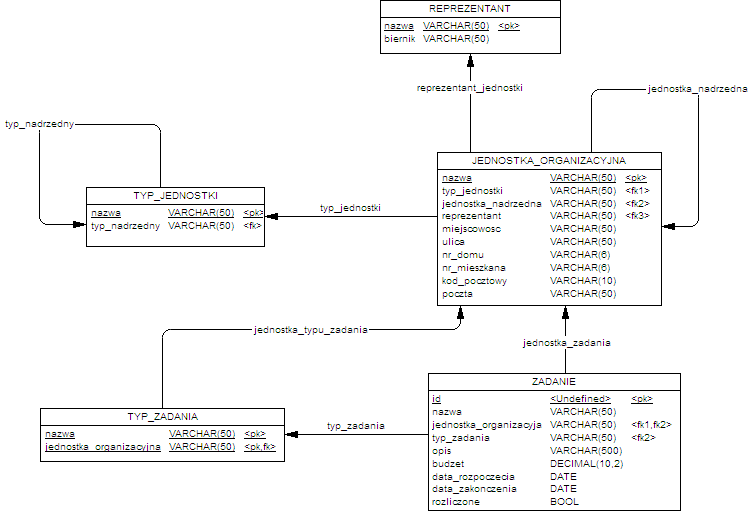
\includegraphics[scale=.8]{img/fizyczny1.png}
	\caption{Diagram fizyczny opisujący strukturę organizacyjną instytucji}
	\label{fizyczny1}
    \end{center}
\end{figure}
\begin{figure}[tdh]
    \begin{center}
	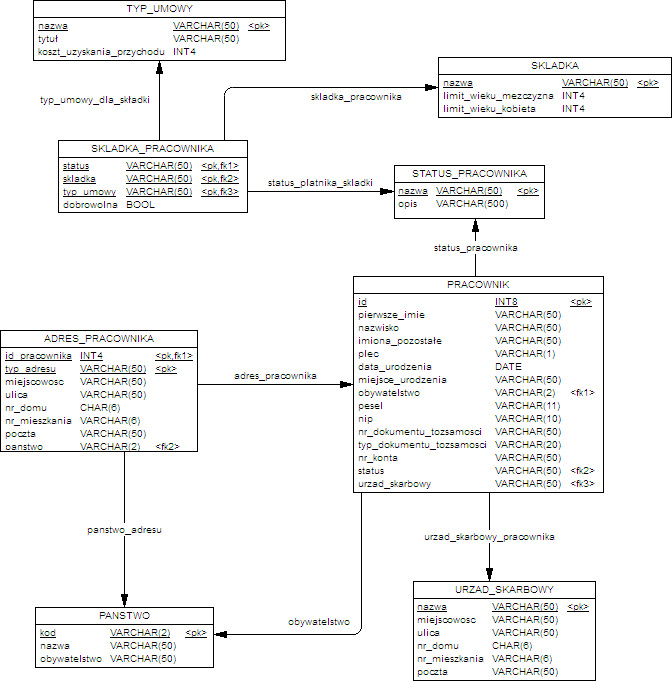
\includegraphics[scale=.8]{img/fizyczny2.png}
	\caption{Diagram fizyczny opisujący pracownika}
	\label{fizyczny2}
    \end{center}
\end{figure}
\begin{figure}[tdh]
    \begin{center}
	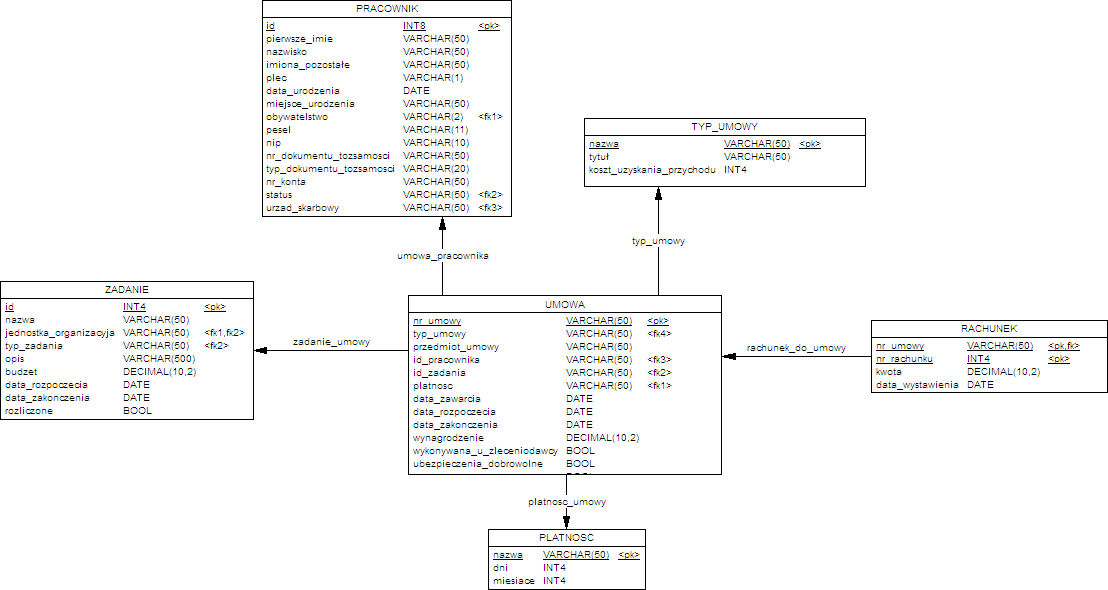
\includegraphics[scale=.8,angle=-90]{img/fizyczny3.png}
	\caption{Diagram fizyczny opisujący umowę}
	\label{fizyczny3}
    \end{center}
\end{figure}

\subsection[Model fizyczny a diagram ER][Model fizyczny a diagram ER]{Model fizyczny a diagram ER}
W projektowanym systemie nie ma dużych różnic pomiędzy modelem fizycznych a diagramem związków encji.
Encje zamieniono na tabele, zaś związki na klucze obce. 

\subsection[Wybór kluczy głównych][Wybór kluczy głównych]{Wybór kluczy głównych}
Jako klucze główne posłużyły unikalne identyfikatory encji. Stało się tak również w przypadkach, w których wybór ten oznaczał pojawienie się klucza złożonego. W przypadkach, w których występowały związki identyfikujące, w skład kluczy złożonych weszły klucze obce.

\subsection[Związki wiele do wielu][Związki wiele do wielu]{Związki wiele do wielu}
Standardowym działaniem podczas przejścia z modelu związków encji do modelu fizycznego jest zamiana binarnych związków wiele do wielu na tabele. W projektowanym systemie takie nie występowały. Pojawił się natomiast związek trynarny. Związki takie są jednak modelowane jako encje już na etapie modelu ER.

